\ifdefined\beamerclass
\else
    \def\beamerclass{beamer}
\fi
\documentclass[\beamerclass]{beamer}

\usepackage{pgfpages}
\mode<handout>{
	% \setbeamercolor{background canvas}{bg=black!20}
	\pgfpagesuselayout{2 on 1}[a4paper,border shrink=5mm]
}


%%%%%%%%%%%%%%%%%%%%%%%%%%%%%%%%%%%%%%%%%%%%%%
% Head matter - can we try to be consistent on
% included packages
%\documentclass{beamer}
\mode<presentation>
{\usetheme{default}
 \usecolortheme{default}
 \usefonttheme{default}
 \setbeamertemplate{navigation symbols}{}
 \setbeamertemplate{footline}[frame number]
% \setbeamertemplate{caption}[numbered]
 }
\usepackage[english]{babel}
\usepackage{algorithm}
\usepackage[noend]{algpseudocode}
\usepackage[utf8x]{inputenc}
\usepackage{graphicx}
\usepackage{hyperref}
%\graphicspath{{./images/}}
\usepackage{tikz}
\usetikzlibrary{shapes.geometric, arrows,chains}
\usepackage{booktabs,makecell,multirow,tabularx}
\usepackage{verbatim}
\renewcommand{\arraystretch}{1.2}
\renewcommand\theadfont{\normalfont\bfseries}
\usepackage{array}
\usepackage{listings}
\lstset{language=Java, showstringspaces=false}
\usepackage[normalem]{ulem}
\usepackage{bm}
\def\layersep{2.5cm}

\usepackage{xcolor}
%\usepackage{subfig}
\setbeamertemplate{caption}{\insertcaption}
\usepackage[caption=false]{subfig}
\usepackage{hyperref}
\usepackage{verbatim}
%\setbeamertemplate{caption}[numbered]%\numberwithin{figure}{section}
% Define block styles
\tikzstyle{decision} = [diamond, draw, fill=blue!20, 
    text width=4.5em, text badly centered, node distance=3cm, inner sep=0pt]
\tikzstyle{block} = [rectangle, draw, fill=blue!20, 
    text width=3em, text centered, rounded corners, minimum height=3em]
\tikzstyle{line} = [draw, -latex']
\tikzstyle{cloud} = [draw, ellipse, fill=red!20, node distance=3cm,
    minimum height=2em]
\tikzset{
  startstop/.style={
    rectangle, 
    rounded corners,
    minimum width=3cm, 
    minimum height=1cm,
    align=center, 
    draw=black, 
    fill=red!30
    },
  process/.style={
    rectangle, 
    minimum width=3cm, 
    minimum height=1cm, 
    align=center, 
    draw=black, 
    fill=blue!30
    },
  decision/.style={
    rectangle, 
    minimum width=3cm, 
    minimum height=1cm, align=center, 
    draw=black, 
    fill=green!30
    },
  arrow/.style={thick,->,>=stealth},
  dec/.style={
    ellipse, 
    align=center, 
    draw=black, 
    fill=green!30
    },
}
\tikzstyle{arrow} = [thick,->,>=stealth]

\tikzset{onslide/.code args={<#1>#2}{%
  \only<#1>{\pgfkeysalso{#2}} % \pgfkeysalso doesn't change the path
}}

\makeatletter
\newenvironment<>{btHighlight}[1][]
{\begin{onlyenv}#2\begingroup\tikzset{bt@Highlight@par/.style={#1}}\begin{lrbox}{\@tempboxa}}
{\end{lrbox}\bt@HL@box[bt@Highlight@par]{\@tempboxa}\endgroup\end{onlyenv}}

\newcommand<>\btHL[1][]{%
  \only#2{\begin{btHighlight}[#1]\bgroup\aftergroup\bt@HL@endenv}%
}
\def\bt@HL@endenv{%
  \end{btHighlight}%   
  \egroup
}
\newcommand{\bt@HL@box}[2][]{%
  \tikz[#1]{%
    \pgfpathrectangle{\pgfpoint{1pt}{0pt}}{\pgfpoint{\wd #2}{\ht #2}}%
    \pgfusepath{use as bounding box}%
    \node[anchor=base west, fill=orange!30,outer sep=0pt,inner xsep=1pt, inner ysep=0pt, rounded corners=3pt, minimum height=\ht\strutbox+1pt,#1]{\raisebox{1pt}{\strut}\strut\usebox{#2}};
  }%
}
\makeatother




%%%%%%%%%%%%%%%%%%%%%%%%%%%%%%%%%%%%%%%%%%%%%%
% Formatting for title page
\title[Deep Learning]{Optimisation}
\author{Kate Farrahi}
\institute{ECS Southampton}
\date{\today}
%%%%%%%%%%%%%%%%%%%%%%%%%%%%%%%%%%%%%%%%%%%%%%
\begin{document}
\begin{frame}
  \titlepage\footnote{Some of the material in this lecture is based on Andrew Ng's lectures on Optimisation} %% \url{https://www.cs.toronto.edu/~tijmen/csc321/slides/lecture_slides_lec6.pdf }} 
\end{frame}
%%-------------------------------------------------------------%


%%-------------------------------------------------------------%
%\begin{frame}[fragile]\frametitle{Multilayer Perceptron}
%\begin{tikzpicture}[shorten >=1pt,->,draw=black!50, node distance=\layersep]
%    \tikzstyle{every pin edge}=[<-,shorten <=1pt]
%    \tikzstyle{neuron}=[circle,fill=black!25,minimum size=17pt,inner sep=0pt]
%    \tikzstyle{input neuron}=[neuron, fill=green!50];
%    \tikzstyle{output neuron}=[neuron, fill=red!50];
%    \tikzstyle{hidden neuron}=[neuron, fill=blue!50];
%    \tikzstyle{annot} = [text width=4em, text centered]
%
%    % Draw the input layer nodes
%    \foreach \name / \y in {1,...,4}
%    % This is the same as writing \foreach \name / \y in {1/1,2/2,3/3,4/4}
%        \node[input neuron] (I-\name) at (0,-\y) {$x_\y$};
%
%    % Draw the hidden layer nodes
%    \foreach \name / \y in {1,...,5}
%        \path[yshift=0.5cm]
%            node[hidden neuron] (H-\name) at (1.5*\layersep,-\y cm) {$h_\y$};
%
%    % Draw the output layer node
%        \foreach \name / \y in {1,...,2}
%        \path[yshift=0.5cm]
%            node[output neuron, pin={[pin edge={->}]right:$y_\y$}, right of=H-3] (O-\name) at (1.5*\layersep,-40-\y cm) {$o_\y$};
%    %\node[output neuron,pin={[pin edge={->}]right:Output}, right of=H-3] (O) {o};
%
%    % Connect every node in the input layer with every node in the
%    % hidden layer.
%    \path (I-1) edge node[anchor=south] {$w_{ji}^{(1)}$}(H-1);
%   \foreach \source in {1,...,4}
%        \foreach \dest in {1,...,5}
%       % \draw [arrow] (I-\source) - (H-\dest);
%            \path (I-\source) edge (H-\dest) ;
%
%    % Connect every node in the hidden layer with the output layer
%    \path (H-1) edge node[anchor=south] {$w_{kj}^{(2)}$}(O-1);
%    \foreach \source in {1,...,5}
%       \foreach \dest in {1,...,2}
%        \path (H-\source) edge (O-\dest);
%
%    % Annotate the layers
%    \node[annot,above of=H-1, node distance=1cm] (hl) {Hidden layer};
%    \node[annot,left of=hl] {Input layer};
%    \node[annot,right of=hl] {Output layer};
%\end{tikzpicture}
%\end{frame}

%-------------------------------------------------------------%


\begin{frame}[fragile]\frametitle{Why learning can be slow}
\hspace{3cm}\centering{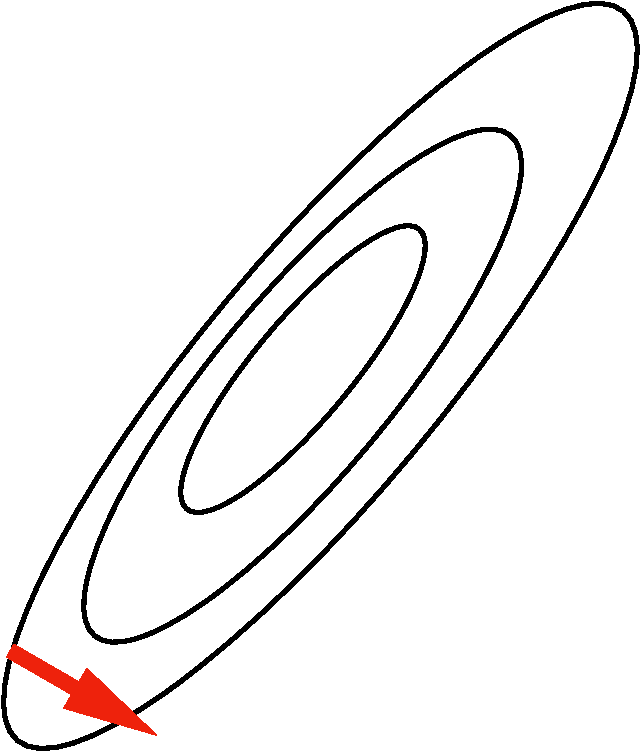
\includegraphics[width=0.5\textwidth]{motivation.pdf}}
\end{frame}
%-------------------------------------------------------------%

\begin{frame}[fragile]\frametitle{Why learning can be slow}

\begin{itemize}
\item If the ellipse is very elongated, the direction of steepest descent is almost perpendicular to the direction towards the minimum
\item The gradient vector will have a large component along the short axis of the ellipse and a small component along the long axis of the ellipse.
\item This is the opposite of what we want to optimise efficiently
\end{itemize}

\end{frame}
%-------------------------------------------------------------%

\begin{frame}{pause}\frametitle{Exponentially Weighted Averages}

$v_t = \beta v_{t-1} + (1 - \beta) \theta_t$ \vspace{3mm} \\ \pause

$v_t$ is approximately average over $\approx \frac{1}{1-\beta}$ days \vspace{6mm} \\ \pause

For example \\
$v_{100} = 0.9 v_{99} + 0.1 \theta_{100}$ \\
$v_{99} = 0.9 v_{98} + 0.1 \theta_{99}$ \\
$v_{98} = 0.9 v_{97} + 0.1 \theta_{98}$ \\
\dots \vspace{3mm} \\ \pause
$v_{100} = 0.1 \theta_{100} + 0.9 [0.1 \theta_{99} + 0.9 [\dots]]]$   \vspace{2mm} \\ \pause
$v_{100} = 0.1 \theta_{100} + 0.9 * 0.1 * \theta_{99} + 0.1 * (0.9)^2 * \theta_{98} + 0.1 (0.9)^3 \theta_{97} + \dots $ 
\end{frame}
%-------------------------------------------------------------%


%\begin{frame}[fragile]\frametitle{ Motivating Momentum}
%\url{https://www.youtube.com/watch?v=7HZk7kGk5bU&t=172s}
%\end{frame}
%-------------------------------------------------------------%

\begin{frame}[fragile]\frametitle{ Momentum}
\begin{itemize}
\item The momentum method allows to accumulate velocity in directions of low curvature that
persist across multiple iterations
\item This leads to accelerated progress in low curvature directions compared to gradient descent %\footnote{\url{http://www.cs.utoronto.ca/~ilya/pubs/ilya_sutskever_phd_thesis.pdf}}
\end{itemize}
\end{frame}
%-------------------------------------------------------------%

\begin{frame}[fragile]\frametitle{ Gradient Descent (GD) with Momentum}

Learning with momentum is given by \vspace{5mm}

On iteration $t$: \\
\hspace{3mm} Compute $dW_t$ on the current mini-batch \\
\begin{eqnarray}
&& V_t =  \beta V_{t-1} + (1 - \beta) dW_{t} \\
&& w_t = w_{t-1} - \eta V_{t}
\end{eqnarray}

Note that $dW_t$ represents the gradient of the cost function (as computed in standard GD). $\eta$ is the learning rate and $\beta = 0.9$ is a good choice for the exponentially weighted average parameter.
\end{frame}
%-------------------------------------------------------------%


\begin{frame}[fragile]\frametitle{RMSProp}
Learning with RMSProp is given by \vspace{5mm}

On iteration $t$: \\
\hspace{3mm} Compute $dW$ on current mini-batch \\
\begin{eqnarray}
&& S_{dW_t} =  \beta S_{dW_{t-1}} + (1 - \beta) dW_t^2 \\
&& w_t = w_{t-1} - \eta \frac{dW_t}{\sqrt S_{dW_t}} 
\end{eqnarray}

\end{frame}
%-------------------------------------------------------------%


\begin{frame}{pause}\frametitle{Bias Correction Motivation}

\begin{itemize}
\item Let's  assume that $v_0 = 0$ and $\beta = 0.9$ and we're considering exponentially weighted averages \pause
\item It follows that $v_1 = \beta (0) + (1 - \beta) \theta_1 = 0.1 \hspace{1mm} \theta_1$  \pause
\item and $v_2 = \beta ( (1 - \beta) \theta_1) + (1-\beta) \theta_2 = 0.0196 \hspace{1mm} \theta_1 + 0.02 \hspace{1mm} \theta_2 $ \pause
\end{itemize}
\end{frame}
%-------------------------------------------------------------%

\begin{frame}{pause}\frametitle{Bias Correction }

\begin{itemize}
\item Add a bias correction term: $\frac{v_t}{1 - \beta^t} $\pause
\item $t = 1$: $\frac{v_1}{1 - (0.9)^1} = 10 * v_1$ \pause
\item $t = 2$: $\frac{v_2}{1 - (0.9)^2} = 5.263 * v_2$ \pause
\item \dots
\item $t = 10$: $\frac{v_{10}}{1 - (0.9)^{10}} = 1.535 * v_{10}$ 
\item \dots
\item $t = 20$: $\frac{v_{20}}{1 - (0.9)^{20}} = 1.138 * v_{20}$ 
\end{itemize}
\end{frame}
%-------------------------------------------------------------%

\begin{frame}[fragile]\frametitle{ Adam}
Initialize parameters: $V_{dW} = 0, S_{dW} = 0$ \vspace{3mm}

On iteration $t$: \\
\hspace{3mm} Compute $dW_t$ on current mini-batch \\
\begin{eqnarray}
&& V_{dW} =  \beta_1 V_{dW} + (1 - \beta_1) dW, \hspace{3mm} V_{dW}^{corr} = \frac{ V_{dW}} { (1 - \beta_1^t)}\\ 
&& S_{dW} =  \beta_2 S_{dW} + (1 - \beta_2) dW^2 , \hspace{3mm} S_{dW}^{corr} = \frac{ S_{dW}} { (1 - \beta_2^t)}\\ 
&& w := w - \eta \frac{V_{dW}^{corr}}{\sqrt (S_{dW}^{corr} + \epsilon)}
\end{eqnarray}

\end{frame}
%-------------------------------------------------------------%


\end{document}
